\documentclass[12pt,a4paper]{article}

% -------------------------------------------------------
% Paquetes
% -------------------------------------------------------
\usepackage[utf8]{inputenc}
\usepackage[spanish]{babel}
\usepackage[T1]{fontenc}
\usepackage{geometry}
\usepackage{graphicx}
\usepackage{xcolor}
\usepackage{listings}
\usepackage{float}
\usepackage{amsmath}
\usepackage{booktabs}
\usepackage{fancyhdr}
\usepackage{titlesec}
\usepackage{setspace}

\geometry{
    top=2.5cm, bottom=2.5cm,
    left=3cm, right=2.5cm
}

% -------------------------------------------------------
% Estilo para codigo C++
% -------------------------------------------------------
\definecolor{codegreen}{rgb}{0,0.55,0}
\definecolor{codegray}{rgb}{0.5,0.5,0.5}
\definecolor{codepurple}{rgb}{0.58,0,0.82}
\definecolor{backcolour}{rgb}{0.97,0.97,0.97}

\lstdefinestyle{estiloCpp}{
    backgroundcolor=\color{backcolour},
    commentstyle=\color{codegreen},
    keywordstyle=\color{blue}\bfseries,
    numberstyle=\tiny\color{codegray},
    stringstyle=\color{codepurple},
    basicstyle=\ttfamily\scriptsize,
    breakatwhitespace=false,
    breaklines=true,
    captionpos=b,
    keepspaces=true,
    numbers=left,
    numbersep=5pt,
    showspaces=false,
    showstringspaces=false,
    showtabs=false,
    tabsize=4,
    language=C++,
    frame=single,
    rulecolor=\color{gray!40},
    xleftmargin=12pt,
    xrightmargin=4pt,
}
\lstset{style=estiloCpp}

% -------------------------------------------------------
% Encabezado y pie de pagina
% -------------------------------------------------------
\pagestyle{fancy}
\fancyhf{}
\fancyhead[L]{\small Computacion Grafica I -- Practica N$^{\circ}$ 07}
\fancyhead[R]{\small Efrain Vitorino Marin}
\fancyfoot[C]{\thepage}
\renewcommand{\headrulewidth}{0.4pt}

% -------------------------------------------------------
% Formato de secciones
% -------------------------------------------------------
\titleformat{\section}{\large\bfseries\color{blue!70!black}}{%
    \thesection.}{0.5em}{}[\titlerule]
\titleformat{\subsection}{\normalsize\bfseries}{\thesubsection.}{0.5em}{}

% -------------------------------------------------------
% Documento
% -------------------------------------------------------
\begin{document}

% ===================================================
% CARATULA
% ===================================================
\thispagestyle{empty}
\begin{center}
    % Logo
    
\includegraphics[width=3.5cm]{logo_unsaac.jpeg}\\[0.4cm]

    {\large\bfseries Universidad Nacional de San Antonio Abad del Cusco}\\[0.2cm]
    {\normalsize Departamento Acad\'emico de Inform\'atica}\\[0.1cm]
    {\normalsize Escuela Profesional: Ing.\ Inform\'atica y de Sistemas}\\[0.8cm]

    \rule{\linewidth}{1.5pt}\\[0.3cm]
    {\Large\bfseries COMPUTACI\'ON GR\'AFICA I}\\[0.2cm]
    \rule{\linewidth}{0.8pt}\\[0.6cm]

    {\LARGE\bfseries Pr\'actica N$^{\circ}$ 07}\\[0.4cm]
    {\Large\bfseries TRANSFORMACI\'ON 2D}\\[0.2cm]
    {\Large\bfseries ESCALA \& ROTACI\'ON}\\[1.2cm]

    \begin{tabular}{rl}
        \textbf{Estudiante:}    & Efrain Vitorino Marin \\[4pt]
        \textbf{C\'odigo:}      & 160337 \\[4pt]
        \textbf{Profesor:}      & Dr.\ Hans Harley Ccacyahuillca Bejar \\[4pt]
        \textbf{Fecha:}         & 1 de junio de 2026 \\
    \end{tabular}

    \vfill
    {\small Cusco -- Per\'u\\2026}
\end{center}

\newpage
\setcounter{page}{1}

% ===================================================
% SECCION 1 — EJERCICIO DEL PDF: ESCALAMIENTO 2D
% ===================================================
\section{Ejercicio 1: Escalamiento 2D}

\subsection{Descripcion}

El programa implementa la transformaci\'on de \textbf{escalamiento homog\'eneo 2D}
mediante matrices $3\times3$ en coordenadas homog\'eneas (column-major de OpenGL).
Se definen tres variantes:

\begin{itemize}
    \item \textbf{Escalamiento con factores independientes} $(s_x, s_y)$:
    \[
    S = \begin{pmatrix} s_x & 0 & 0 \\ 0 & s_y & 0 \\ 0 & 0 & 1 \end{pmatrix}
    \]

    \item \textbf{Escalamiento alrededor de un punto} $(c_x, c_y)$:
    la transformaci\'on combinada $T(c_x,c_y)\cdot S(s_x,s_y)\cdot T(-c_x,-c_y)$
    produce la matriz:
    \[
    S_c = \begin{pmatrix}
        s_x & 0   & c_x(1-s_x) \\
        0   & s_y & c_y(1-s_y) \\
        0   & 0   & 1
    \end{pmatrix}
    \]

    \item \textbf{Escalamiento uniforme}: caso particular con $s_x = s_y = s$.
\end{itemize}

Se renderiza un cuadrado centrado en el origen con una cruz interna.
Los controles son: \texttt{Q}/\texttt{A} (escala X), \texttt{W}/\texttt{S} (escala Y),
\texttt{E}/\texttt{D} (escala uniforme), \texttt{R} (reiniciar), \texttt{ESC} (salir).

\subsection{Resultado en consola}

\begin{verbatim}
=== CONTROLES ===
Q / A: Aumentar / Disminuir escala en X
W / S: Aumentar / Disminuir escala en Y
E / D: Aumentar / Disminuir escala uniforme
R: Reiniciar escalas
ESC: Salir
=================
Escala X: 1 | Escala Y: 1 | Escala Uniforme: 1
Escala X: 1 | Escala Y: 1 | Escala Uniforme: 1
\end{verbatim}

\subsection{Captura de pantalla}

\begin{figure}[H]
    \centering
    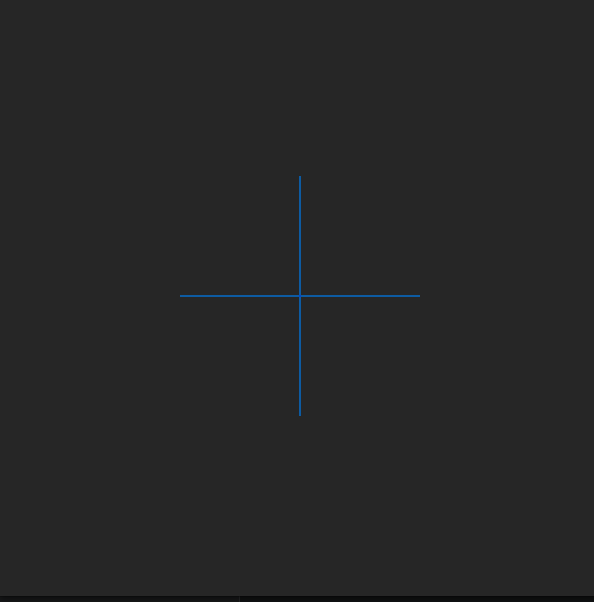
\includegraphics[width=0.6\textwidth]{escalamiento_resultado.png}
    \caption{Ventana \texttt{escalamiento}: cuadrado con cruz de referencia
    (solo la cr\texttt{u}z GL\_LINES es visible en Core Profile).}
\end{figure}

\newpage

% ===================================================
% SECCION 2 — EJERCICIO DEL PDF: ROTACION 2D
% ===================================================
\section{Ejercicio 2: Rotaci\'on 2D}

\subsection{Descripcion}

El programa implementa la transformaci\'on de \textbf{rotaci\'on 2D} alrededor
del origen y alrededor de un punto arbitrario $(c_x, c_y)$, usando matrices $3\times3$.

\begin{itemize}
    \item \textbf{Rotaci\'on alrededor del origen} (\'angulo $\theta$):
    \[
    R(\theta) = \begin{pmatrix}
        \cos\theta & -\sin\theta & 0 \\
        \sin\theta &  \cos\theta & 0 \\
        0          & 0           & 1
    \end{pmatrix}
    \]

    \item \textbf{Rotaci\'on alrededor de un punto} $(c_x, c_y)$:
    la transformaci\'on $T(c)\cdot R(\theta)\cdot T(-c)$ da:
    \[
    R_c = \begin{pmatrix}
        \cos\theta & -\sin\theta & c_x - c_x\cos\theta + c_y\sin\theta \\
        \sin\theta &  \cos\theta & c_y - c_x\sin\theta - c_y\cos\theta \\
        0          & 0           & 1
    \end{pmatrix}
    \]
\end{itemize}

Se dibuja un tri\'angulo en tres versiones: original (rojo), rotado alrededor
del origen (verde), rotado a $1.5\theta$ alrededor del centroide (azul).
Controles: \texttt{R} (girar $+$), \texttt{T} (girar $-$), \texttt{ESC} (salir).

\subsection{Resultado en consola}

\begin{verbatim}
Angulo de rotacion (verde): 0 grados
Angulo de rotacion (verde): 13 grados
Angulo de rotacion (verde): 25 grados
Angulo de rotacion (verde): 4 grados
Angulo de rotacion (verde): -22 grados
Angulo de rotacion (verde): -33 grados
\end{verbatim}

\subsection{Captura de pantalla}

\begin{figure}[H]
    \centering
    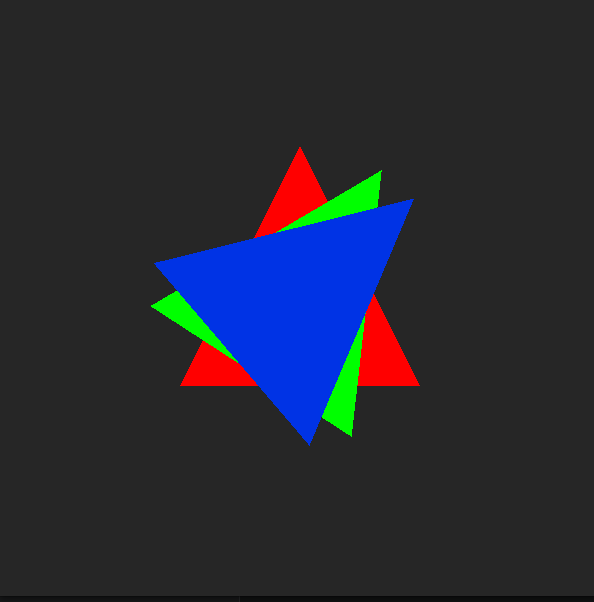
\includegraphics[width=0.6\textwidth]{rotacion_resultado.png}
    \caption{Ventana \texttt{rotacion}: tri\'angulo original (rojo), rotado
    respecto al origen (verde) y rotado respecto al centroide a $1.5\theta$ (azul).}
\end{figure}

\newpage

% ===================================================
% SECCION 3 — ACTIVIDAD 1: ESCALAMIENTO DE CIRCULO
% ===================================================
\section{Actividad 1: Escalamiento de C\'irculo}

\subsection{Enunciado}

\textit{``Escribir un programa que escale un c\'irculo dos veces su
dimensi\'on original manteniendo fijo su centro.''}

\subsection{Descripcion de la solucion}

Se genera un c\'irculo usando \texttt{GL\_TRIANGLE\_FAN} con 64 segmentos,
centrado en el origen con radio $r = 0.3$. El escalamiento $\times 2$
con centro fijo se obtiene con:
\[
S_c(2, 2, 0, 0) = \begin{pmatrix} 2 & 0 & 0 \\ 0 & 2 & 0 \\ 0 & 0 & 1 \end{pmatrix}
\]
Como el centro es el origen, la traslaci\'on compensatoria es nula y la
matriz coincide con el escalamiento simple. El c\'irculo blanco es el original
y el verde es el escalado.

\subsection{Codigo fuente}

\begin{lstlisting}[caption={actividadCirculo.cpp}]
#include <GL/glew.h>
#include <GLFW/glfw3.h>
#include <glm/glm.hpp>
#include <glm/gtc/type_ptr.hpp>
#include <iostream>
#include <string>
#include <cmath>
#include <vector>

const char* vertSrc = R"(
#version 330 core
layout(location = 0) in vec2 aPos;
uniform mat3 uTransform;
void main() {
    vec3 p = uTransform * vec3(aPos, 1.0);
    gl_Position = vec4(p.xy, 0.0, 1.0);
}
)";

const char* fragSrc = R"(
#version 330 core
uniform vec4 uColor;
out vec4 fragColor;
void main() { fragColor = uColor; }
)";

GLuint shaderProg, vao, vbo;
int numVerticesCirculo = 0;
const float CENTRO_X = 0.0f, CENTRO_Y = 0.0f, RADIO = 0.3f;

void matrizIdentidad(float M[9]) {
    M[0]=1; M[3]=0; M[6]=0;
    M[1]=0; M[4]=1; M[7]=0;
    M[2]=0; M[5]=0; M[8]=1;
}

void matrizEscalamientoAlrededorDe(float sx,float sy,float cx,float cy,float M[9]){
    float tx = cx - sx*cx, ty = cy - sy*cy;
    M[0]=sx; M[3]=0;  M[6]=tx;
    M[1]=0;  M[4]=sy; M[7]=ty;
    M[2]=0;  M[5]=0;  M[8]=1;
}

void inicializarGeometria() {
    const int segmentos = 64;
    std::vector<float> v;
    v.push_back(CENTRO_X); v.push_back(CENTRO_Y);
    for (int i = 0; i <= segmentos; i++) {
        float a = 2.0f * M_PI * i / segmentos;
        v.push_back(CENTRO_X + RADIO * cos(a));
        v.push_back(CENTRO_Y + RADIO * sin(a));
    }
    numVerticesCirculo = (int)(v.size() / 2);
    glGenVertexArrays(1, &vao); glGenBuffers(1, &vbo);
    glBindVertexArray(vao);
    glBindBuffer(GL_ARRAY_BUFFER, vbo);
    glBufferData(GL_ARRAY_BUFFER, v.size()*sizeof(float), v.data(), GL_STATIC_DRAW);
    glVertexAttribPointer(0,2,GL_FLOAT,GL_FALSE,2*sizeof(float),(void*)0);
    glEnableVertexAttribArray(0);
    glBindVertexArray(0);
}

int main() {
    glfwInit();
    glfwWindowHint(GLFW_CONTEXT_VERSION_MAJOR, 3);
    glfwWindowHint(GLFW_CONTEXT_VERSION_MINOR, 3);
    glfwWindowHint(GLFW_OPENGL_PROFILE, GLFW_OPENGL_CORE_PROFILE);
    GLFWwindow* window = glfwCreateWindow(600,600,
        "Actividad 1 - Escalamiento de circulo", NULL, NULL);
    glfwMakeContextCurrent(window);
    glewExperimental = GL_TRUE; glewInit();
    glClearColor(0.15f,0.15f,0.15f,1.0f);
    glEnable(GL_BLEND); glBlendFunc(GL_SRC_ALPHA, GL_ONE_MINUS_SRC_ALPHA);
    // compilarShaders(...) omitido por brevedad
    inicializarGeometria();
    GLint locMat = glGetUniformLocation(shaderProg,"uTransform");
    GLint locColor = glGetUniformLocation(shaderProg,"uColor");
    float M[9];
    while (!glfwWindowShouldClose(window)) {
        if (glfwGetKey(window, GLFW_KEY_ESCAPE)==GLFW_PRESS)
            glfwSetWindowShouldClose(window,true);
        glClear(GL_COLOR_BUFFER_BIT);
        glUseProgram(shaderProg);
        glBindVertexArray(vao);
        // Circulo original (blanco)
        matrizIdentidad(M);
        glUniformMatrix3fv(locMat,1,GL_FALSE,M);
        glUniform4f(locColor, 1.0f, 1.0f, 1.0f, 0.6f);
        glDrawArrays(GL_TRIANGLE_FAN, 0, numVerticesCirculo);
        // Circulo escalado x2, centro fijo (verde)
        matrizEscalamientoAlrededorDe(2.0f,2.0f,CENTRO_X,CENTRO_Y,M);
        glUniformMatrix3fv(locMat,1,GL_FALSE,M);
        glUniform4f(locColor, 0.0f, 1.0f, 0.0f, 0.5f);
        glDrawArrays(GL_TRIANGLE_FAN, 0, numVerticesCirculo);
        glBindVertexArray(0);
        glfwSwapBuffers(window); glfwPollEvents();
    }
    glDeleteVertexArrays(1,&vao); glDeleteBuffers(1,&vbo);
    glDeleteProgram(shaderProg);
    glfwDestroyWindow(window); glfwTerminate();
    return 0;
}
\end{lstlisting}

\subsection{Resultado en consola}

\begin{verbatim}
=== Actividad 1: Escalar circulo x2 manteniendo centro fijo ===
Blanco: circulo original  (radio 0.3)
Verde:  circulo escalado x2 con centro fijo en (0, 0)
ESC: Salir
\end{verbatim}

\subsection{Captura de pantalla}

\begin{figure}[H]
    \centering
    
\includegraphics[width=0.6\textwidth]{circulo_resultado.png}
    \caption{Actividad 1: c\'irculo blanco (original, radio $= 0.3$) y c\'irculo
    verde escalado $\times 2$ (radio $= 0.6$) con centro fijo en el origen.}
\end{figure}

\newpage

% ===================================================
% SECCION 4 — ACTIVIDAD 2: TRASLACION Y ROTACION
% ===================================================
\section{Actividad 2: Traslaci\'on y Rotaci\'on de Rect\'angulo}

\subsection{Enunciado}

\textit{``Realizar una traslaci\'on y luego una rotaci\'on de un rect\'angulo.''}

\subsection{Descripcion de la solucion}

Se define un rect\'angulo centrado en el origen ($0.6 \times 0.3$ unidades).
La transformaci\'on combina:
\begin{enumerate}
    \item \textbf{Traslaci\'on} $T(0.4,\;0.2)$
    \item \textbf{Rotaci\'on} $R(\theta)$ alrededor del origen
\end{enumerate}

La matriz combinada es $M = R(\theta)\cdot T(0.4,\,0.2)$, obtenida con la funci\'on
\texttt{multiplicarMatrices(R, T, TR)}. Al aplicarse de derecha a izquierda,
primero se traslada el rect\'angulo y luego se rota el resultado.

La f\'ormula matem\'atica es:
\[
M = R(\theta)\cdot T = \begin{pmatrix}
    \cos\theta & -\sin\theta & 0.4\cos\theta - 0.2\sin\theta \\
    \sin\theta &  \cos\theta & 0.4\sin\theta + 0.2\cos\theta \\
    0 & 0 & 1
\end{pmatrix}
\]

Controles: \texttt{R} (girar $+$), \texttt{T} (girar $-$), \texttt{ESC} (salir).

\subsection{Codigo fuente}

\begin{lstlisting}[caption={actividadRectangulo.cpp}]
#include <GL/glew.h>
#include <GLFW/glfw3.h>
#include <glm/glm.hpp>
#include <glm/gtc/type_ptr.hpp>
#include <iostream>
#include <string>
#include <cmath>

const char* vertSrc = R"(
#version 330 core
layout(location = 0) in vec2 aPos;
uniform mat3 uTransform;
void main() {
    vec3 p = uTransform * vec3(aPos, 1.0);
    gl_Position = vec4(p.xy, 0.0, 1.0);
}
)";
const char* fragSrc = R"(
#version 330 core
uniform vec4 uColor;
out vec4 fragColor;
void main() { fragColor = uColor; }
)";

GLuint shaderProg, vao, vbo;

void matrizIdentidad(float M[9]) {
    M[0]=1;M[3]=0;M[6]=0; M[1]=0;M[4]=1;M[7]=0; M[2]=0;M[5]=0;M[8]=1;
}
void matrizTraslacion(float tx, float ty, float M[9]) {
    M[0]=1; M[3]=0; M[6]=tx;
    M[1]=0; M[4]=1; M[7]=ty;
    M[2]=0; M[5]=0; M[8]=1;
}
void matrizRotacion(float anguloGrados, float M[9]) {
    float rad = anguloGrados * M_PI / 180.0f;
    float c = cos(rad), s = sin(rad);
    M[0]= c; M[3]=-s; M[6]=0;
    M[1]= s; M[4]= c; M[7]=0;
    M[2]=0;  M[5]=0;  M[8]=1;
}
// C = A * B  (aplica B primero, luego A)
void multiplicarMatrices(const float A[9], const float B[9], float C[9]) {
    for (int col=0; col<3; col++)
        for (int f=0; f<3; f++)
            C[col*3+f] = A[0*3+f]*B[col*3+0]
                       + A[1*3+f]*B[col*3+1]
                       + A[2*3+f]*B[col*3+2];
}

void inicializarGeometria() {
    float v[] = {
        -0.3f, 0.15f,   0.3f, 0.15f,  0.3f,-0.15f,
        -0.3f, 0.15f,   0.3f,-0.15f, -0.3f,-0.15f
    };
    glGenVertexArrays(1,&vao); glGenBuffers(1,&vbo);
    glBindVertexArray(vao);
    glBindBuffer(GL_ARRAY_BUFFER,vbo);
    glBufferData(GL_ARRAY_BUFFER,sizeof(v),v,GL_STATIC_DRAW);
    glVertexAttribPointer(0,2,GL_FLOAT,GL_FALSE,2*sizeof(float),(void*)0);
    glEnableVertexAttribArray(0);
    glBindVertexArray(0);
}

int main() {
    glfwInit();
    glfwWindowHint(GLFW_CONTEXT_VERSION_MAJOR,3);
    glfwWindowHint(GLFW_CONTEXT_VERSION_MINOR,3);
    glfwWindowHint(GLFW_OPENGL_PROFILE,GLFW_OPENGL_CORE_PROFILE);
    GLFWwindow* window = glfwCreateWindow(600,600,
        "Actividad 2 - Traslacion y Rotacion de rectangulo",NULL,NULL);
    glfwMakeContextCurrent(window);
    glewExperimental=GL_TRUE; glewInit();
    glClearColor(0.15f,0.15f,0.15f,1.0f);
    glEnable(GL_BLEND); glBlendFunc(GL_SRC_ALPHA,GL_ONE_MINUS_SRC_ALPHA);
    // compilarShaders(...) omitido por brevedad
    inicializarGeometria();
    GLint locMat   = glGetUniformLocation(shaderProg,"uTransform");
    GLint locColor = glGetUniformLocation(shaderProg,"uColor");
    float M[9], T[9], R[9], TR[9];
    float angulo = 0.0f;
    const float TX=0.4f, TY=0.2f;
    while (!glfwWindowShouldClose(window)) {
        if (glfwGetKey(window,GLFW_KEY_ESCAPE)==GLFW_PRESS)
            glfwSetWindowShouldClose(window,true);
        if (glfwGetKey(window,GLFW_KEY_R)==GLFW_PRESS) angulo += 1.0f;
        if (glfwGetKey(window,GLFW_KEY_T)==GLFW_PRESS) angulo -= 1.0f;
        glClear(GL_COLOR_BUFFER_BIT);
        glUseProgram(shaderProg);
        glBindVertexArray(vao);
        // Rectangulo original (rojo)
        matrizIdentidad(M);
        glUniformMatrix3fv(locMat,1,GL_FALSE,M);
        glUniform4f(locColor,1,0,0,0.6f);
        glDrawArrays(GL_TRIANGLES,0,6);
        // Rectangulo trasladado + rotado (verde)
        // M = R * T  => aplica T primero, luego R
        matrizTraslacion(TX,TY,T);
        matrizRotacion(angulo,R);
        multiplicarMatrices(R,T,TR);
        glUniformMatrix3fv(locMat,1,GL_FALSE,TR);
        glUniform4f(locColor,0,1,0,0.7f);
        glDrawArrays(GL_TRIANGLES,0,6);
        glBindVertexArray(0);
        glfwSwapBuffers(window); glfwPollEvents();
    }
    glDeleteVertexArrays(1,&vao); glDeleteBuffers(1,&vbo);
    glDeleteProgram(shaderProg);
    glfwDestroyWindow(window); glfwTerminate();
    return 0;
}
\end{lstlisting}

\subsection{Resultado en consola}

\begin{verbatim}
=== Actividad 2: Traslacion + Rotacion de rectangulo ===
Rojo:  rectangulo original en el origen
Verde: rectangulo trasladado (0.4, 0.2) y luego rotado
R: Aumentar angulo | T: Disminuir angulo | ESC: Salir
Angulo de rotacion: 0 grados
Angulo de rotacion: 12 grados
Angulo de rotacion: 28 grados
Angulo de rotacion: -20 grados
Angulo de rotacion: -80 grados
Angulo de rotacion: -140 grados
Angulo de rotacion: -144 grados
Angulo de rotacion: -119 grados
\end{verbatim}

\subsection{Captura de pantalla}

\begin{figure}[H]
    \centering
    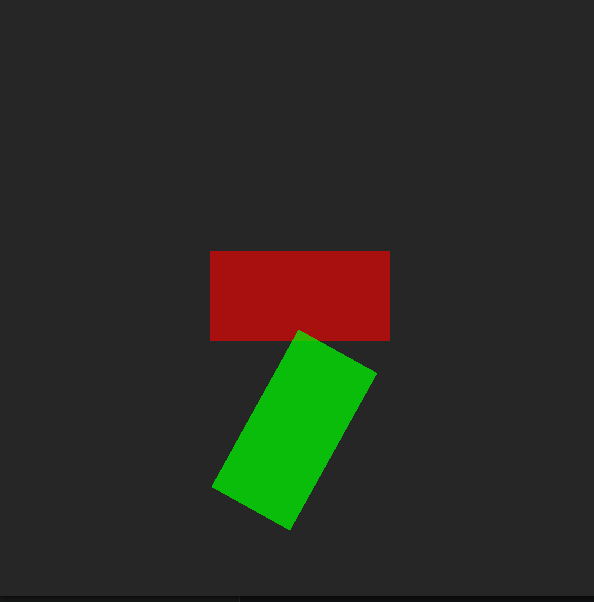
\includegraphics[width=0.6\textwidth]{rectangulo_resultado.png}
    \caption{Actividad 2: rect\'angulo rojo (posici\'on original en el origen)
    y rect\'angulo verde (trasladado a $(0.4,\,0.2)$ y rotado $\theta\approx-119^\circ$).}
\end{figure}

\end{document}
